\documentclass{article}
\usepackage{graphicx} % Required for inserting images
\usepackage{float}
\usepackage[T1]{fontenc}
\usepackage{amsmath}
\usepackage[margin=1in]{geometry}
\usepackage{booktabs}
\usepackage{tabularx}
\usepackage[hidelinks]{hyperref}

\title{Hedging half the delta of high-VRP puts on the stress-sized SPY put book}
\author{Experiment report \textperiodcentered{} L/S Gamma Desk, QUANTT}
\date{2026-11-02}

\begin{document}

\maketitle

\textbf{Question:} On the 35\% stress-sized \texttt{hedged} put book, does hedging only half the delta of a put entered when VRP is above 2 vol points, while keeping the book's full size, earn more than always hedging, with a better Sharpe ratio and a drawdown within the stress budget?

\textbf{Method:}

\begin{itemize}

\item \textbf{Pre-registration.} The hypothesis card was committed before any run (commit 79b09a1).

\item \textbf{Data and book.} The 2026-10-22 \texttt{hedged} book is replayed on R2 replay snapshots v1 (config\_hash b040760187f0) over the development window 2014-06-02 to 2024-12-31. The hold-out (2025-01-01 to 2026-07-10) was not used.

\begin{itemize}

\item The book is an always-on short 25-delta put, sized at entry to a 35\% stress budget: a one-day 20\% drop with IV at max(60\%, the put's IV) may cost at most \$87,500.

\item It is hedged daily at 10:15 with a 10-share band.

\end{itemize}

\item \textbf{New switch.} Research-only \texttt{[backtest] vrp\_\allowbreak{}hedge\_\allowbreak{}cut} and \texttt{vrp\_\allowbreak{}hedge\_\allowbreak{}ratio}. A put entered when VRP (ATM IV minus the GARCH forecast, at the 10:15 decision) is above the cutoff has its hedge target multiplied by the ratio for its whole life.

\begin{itemize}

\item Its size is the hedged book's full size: the stress test ignores the delta left unhedged. That was the PM's choice, so this card tests only the hedge.

\end{itemize}

\item \textbf{Variants:} \texttt{half2} = cutoff 0.02 (the live short band), ratio 0.5 (primary); \texttt{none2} = cutoff 0.02, ratio 0; \texttt{half1} = cutoff 0.01, ratio 0.5.

\item \textbf{Reference.} The registered \texttt{2026-\allowbreak{}10-\allowbreak{}22-\allowbreak{}stress-\allowbreak{}sized-\allowbreak{}puts/\allowbreak{}hedged} runs, reused and not rerun, at the same spread multiple. The registered \texttt{2026-\allowbreak{}11-\allowbreak{}02-\allowbreak{}vrp-\allowbreak{}hedge/\allowbreak{}vrp2} book (fully unhedged above 2 points, at the smaller unhedged size) is shown for context.

\item \textbf{Runs and costs.} Every variant was run at 1x and 2x spreads. Costs are \$0.65 per contract and \$0.005 per share, with a \$1 minimum per order. Exits and hedges run at 10:15 ET.

\end{itemize}

\section{Result vs the pass bar}

Every check had to hold at 1x and 2x. P\&L is net of spreads and commissions, in USD, for the sized book.

\begin{center}\small
\begin{tabularx}{\linewidth}{>{\raggedright\arraybackslash}X l l l l l}
\toprule
\textbf{Check (\texttt{half2} vs \texttt{hedged})} & \textbf{1x value} & \textbf{1x bar} & \textbf{2x value} & \textbf{2x bar} & \textbf{Result} \\
\midrule
Net P\&L, full window & \$142,653 & > \$121,482 & \$117,002 & > \$101,172 & pass \\
Net P\&L, 2014-06 to 2019-12 & \$64,611 & > \$49,132 & \$54,135 & > \$42,687 & pass \\
Net P\&L, 2020-01 to 2024-12 & \$78,041 & > \$72,350 & \$62,868 & > \$58,485 & pass \\
Sharpe ratio, full window & 0.50 & > 0.52 & 0.41 & > 0.43 & fail \\
Max drawdown & \$98,210 & \ensuremath{\leq} \$87,500 & \$105,611 & \ensuremath{\leq} \$87,500 & fail \\
Partly hedged round trips (floor \ensuremath{\geq} 20, 1x) & 38 &  &  &  & met \\
\bottomrule
\end{tabularx}
\end{center}

\textbf{Verdict: failed.} The half hedge made more money than always hedging: \$21.2k more at 1x and \$15.8k more at 2x, in both halves. But it failed the risk checks:

\begin{itemize}

\item its Sharpe ratio was slightly lower;

\item its drawdown broke the \$87,500 stress budget at both spreads.

\end{itemize}

Almost all of the extra risk comes from one partly hedged put entered on 2 March 2020.

\subsection{Full-window numbers (not part of the bar)}

\begin{center}\small
\begin{tabularx}{\linewidth}{>{\raggedright\arraybackslash}X >{\raggedright\arraybackslash}X >{\raggedright\arraybackslash}X >{\raggedright\arraybackslash}X >{\raggedright\arraybackslash}X >{\raggedright\arraybackslash}X >{\raggedright\arraybackslash}X}
\toprule
\textbf{} & \textbf{\texttt{hedged} 1x} & \textbf{\texttt{vrp2} 1x} & \textbf{\texttt{half2} 1x} & \textbf{\texttt{none2} 1x} & \textbf{\texttt{half1} 1x} & \textbf{\texttt{half2} 2x} \\
\midrule
Net P\&L & \$121,482 & \$114,100 & \$142,653 & \$168,561 & \$188,041 & \$117,002 \\
Sharpe & 0.52 & 0.51 & 0.50 & 0.64 & 0.65 & 0.41 \\
Max drawdown & \$70,362 & \$73,622 & \$98,210 & \$84,054 & \$74,528 & \$105,611 \\
ES 5\% (daily) & \ensuremath{-}\$3,016 & \ensuremath{-}\$3,373 & \ensuremath{-}\$3,813 & \ensuremath{-}\$3,888 & \ensuremath{-}\$3,918 & \ensuremath{-}\$3,936 \\
Round trips & 182 & 208 & 195 & 208 & 196 & 195 \\
Commissions (options /\allowbreak{} hedges) & \$5,955 /\allowbreak{} \$2,868 & \$6,300 /\allowbreak{} \$2,671 & \$6,378 /\allowbreak{} \$2,820 & \$6,789 /\allowbreak{} \$2,686 & \$6,440 /\allowbreak{} \$2,777 & \$6,380 /\allowbreak{} \$2,818 \\
\bottomrule
\end{tabularx}
\end{center}

Both sensitivities cleared every check of this card at both spreads:

\begin{itemize}

\item \texttt{none2}: \$168.6k and \$144.6k; Sharpe 0.64 and 0.53; drawdown \$84.1k and \$86.1k.

\item \texttt{half1}: \$188.0k and \$168.4k; Sharpe 0.65 and 0.57; drawdown \$74.5k and \$75.8k.

\end{itemize}

Sensitivities cannot pass a card. As the analysis shows, the gaps between the three variants come mostly from different paths through March 2020.

\section{Charts}

\begin{figure}[H]\centering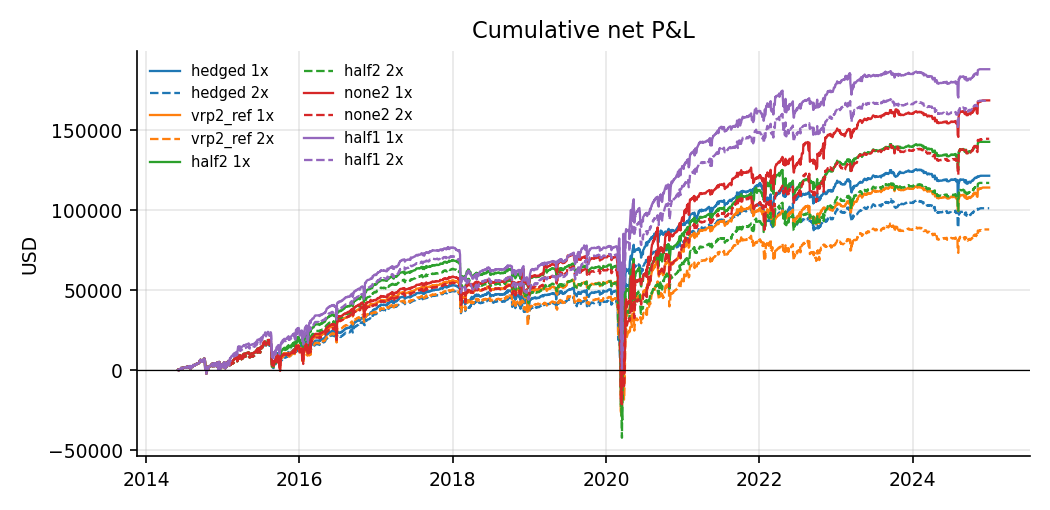
\includegraphics[width=0.92\linewidth]{figures/cum_pnl.png}\caption{Cumulative net P\&L, 1x solid and 2x dashed; vrp2\_ref is the fully unhedged 2026-11-02 book}\end{figure}

\texttt{half1} pulls ahead of the hedged book from 2015; \texttt{half2} and \texttt{none2} from 2016. In March 2020 \texttt{half2} falls furthest, to \ensuremath{-}\$29.4k cumulative at 1x and \ensuremath{-}\$42.2k at 2x on 17 March, then recovers. It has stayed above \texttt{hedged} since January 2022 at 1x and November 2022 at 2x.

\begin{figure}[H]\centering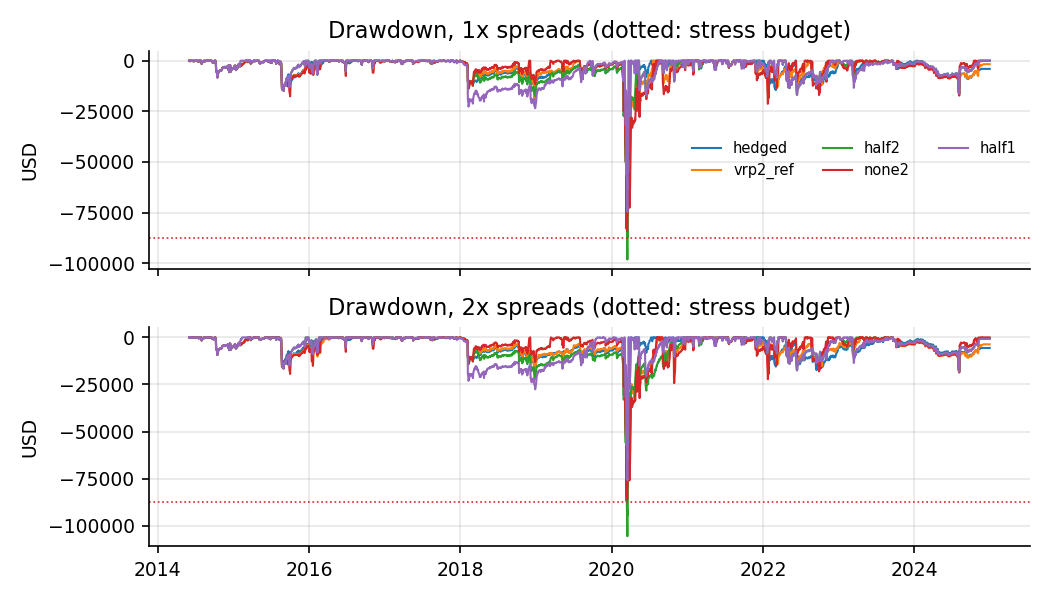
\includegraphics[width=0.92\linewidth]{figures/drawdown.png}\caption{Drawdown at 1x and 2x spreads; dotted line: the \$87,500 stress budget}\end{figure}

Every book's worst drawdown ends on 16 or 17 March 2020. \texttt{half2} is the only book below the budget line at both spreads. \texttt{none2} comes within about \$1.5k of it at 2x.

\begin{figure}[H]\centering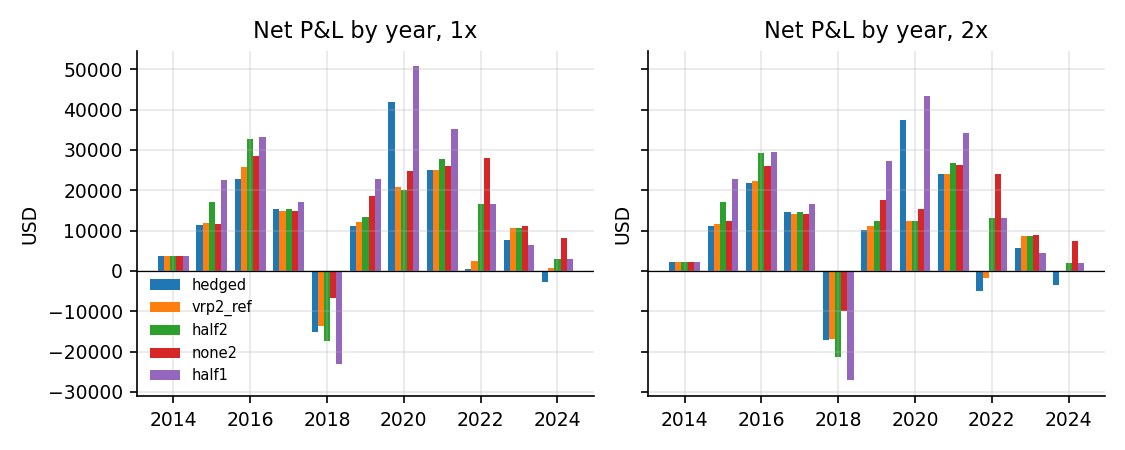
\includegraphics[width=0.92\linewidth]{figures/yearly.png}\caption{Net P\&L by year}\end{figure}

At 1x, \texttt{half2} beat \texttt{hedged} in seven of the nine years where they differ, and trailed in 2018 (\ensuremath{-}\$2.2k) and 2020 (\ensuremath{-}\$21.8k). 2014 and 2017 had no partly hedged entries and are identical. The largest gain is 2022 (+\$16.2k, from 5 partly hedged entries).

\begin{figure}[H]\centering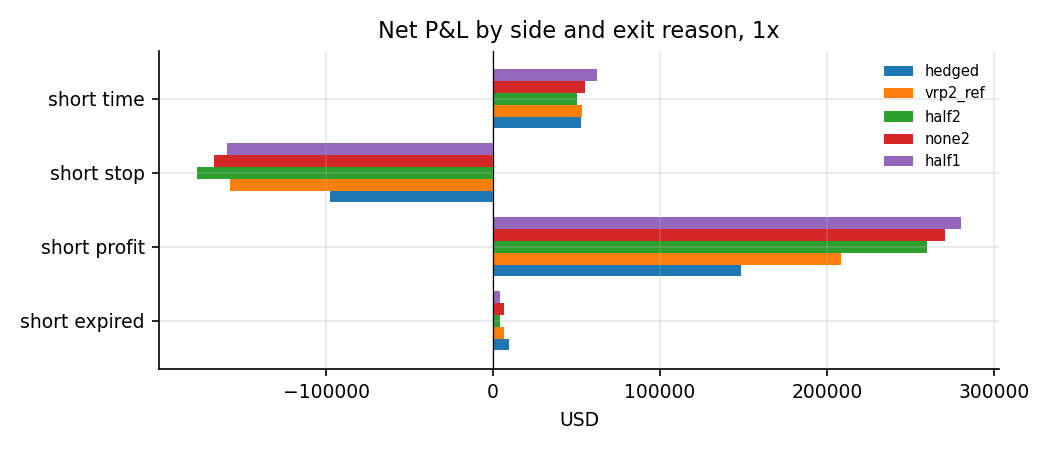
\includegraphics[width=0.92\linewidth]{figures/by_reason.png}\caption{Net P\&L by side and exit reason, 1x}\end{figure}

Partly hedged puts take profits much more often. Within \texttt{half2}:

\begin{itemize}

\item \textbf{Partly hedged puts:} 22 of 38 closed at the 50\% profit-take, for \$128.2k.

\item \textbf{Fully hedged puts:} 21 of 157, for \$131.8k.

\end{itemize}

When SPY rises, the delta left unhedged adds to the put's P\&L, so the profit-take is reached sooner. Five partly hedged puts were stopped, for \ensuremath{-}\$92.6k.

\begin{figure}[H]\centering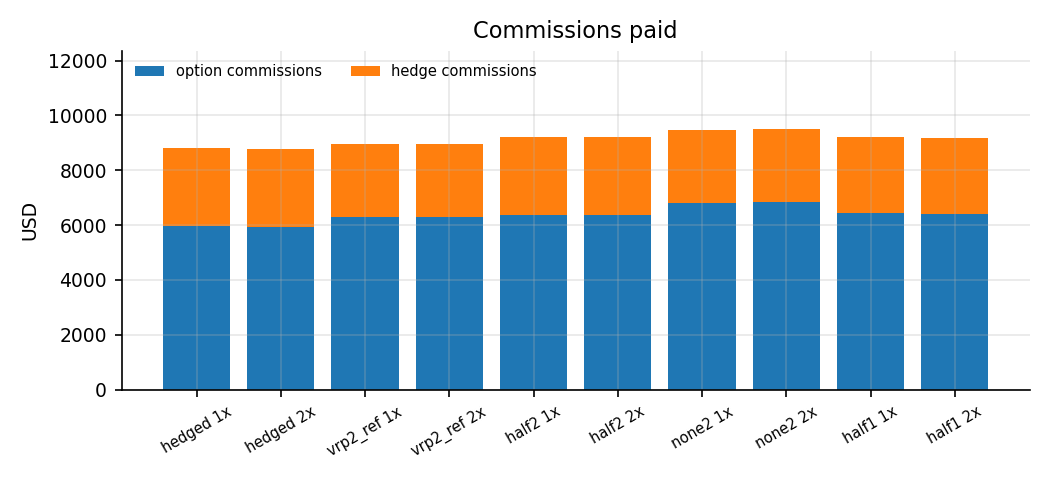
\includegraphics[width=0.92\linewidth]{figures/fees.png}\caption{Commissions paid}\end{figure}

Commissions barely move: \texttt{half2} paid \$9.2k in total at 1x against \$8.8k for \texttt{hedged}. A half hedge still trades shares every day, so hedge commissions fall only slightly (\$2,820 against \$2,868).

\begin{figure}[H]\centering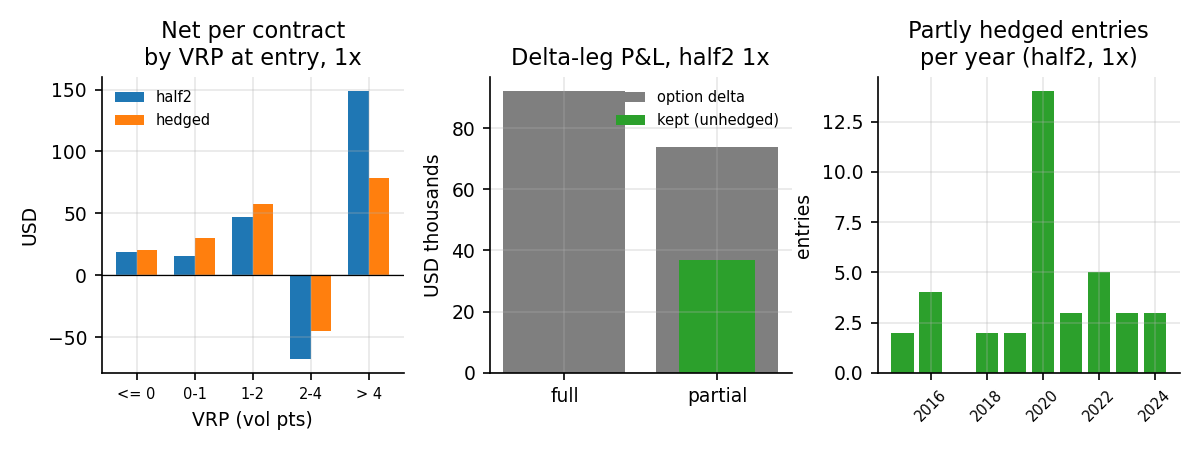
\includegraphics[width=0.92\linewidth]{figures/mechanism.png}\caption{Mechanism: net per contract by VRP at entry (1x); delta-leg P\&L of fully and partly hedged puts in half2 (1x); partly hedged entries per year}\end{figure}

\begin{itemize}

\item \textbf{Left panel:} above 4 vol points, \texttt{half2} made \$149 per contract (pooled) against \$78 for \texttt{hedged}. In the 2-4 point bucket both lose, \texttt{half2} more (\ensuremath{-}\$68 against \ensuremath{-}\$45), and that bucket holds the 2 March 2020 put.

\item \textbf{Middle panel:} the delta of the 38 partly hedged puts earned \$73.9k over 381 position-days, 30\% a year per dollar of delta held. The 157 fully hedged puts' delta earned 7\% a year. The half left unhedged kept \$36.9k of it.

\item \textbf{Right panel:} 14 of the 38 partly hedged entries were in 2020, most of them after the crash.

\end{itemize}

\section{Analysis}

\textbf{The timing still shows up in the delta leg.} Puts entered above 2 VRP points had a delta that paid about four times as much per dollar as the others:

\begin{itemize}

\item \textbf{This card:} 30\% a year against 7\%, measured as snapshot delta times the spot change between 10:15 decisions.

\item \textbf{\texttt{vrp-\allowbreak{}hedge}:} the same split showed 64\% against 9.5\% in the always-unhedged 2026-10-22 book.

\end{itemize}

Partly hedged puts made \$52.6 per contract pooled (38 round trips) against \$21.5 for fully hedged ones (157). Without the 2 March 2020 put, the other 37 partly hedged round trips made \$108.3k, and 32 of them were profitable.

Keeping full size worked as intended: partly hedged puts averaged 26.6 contracts against 24.9 for fully hedged puts. In \texttt{vrp-\allowbreak{}hedge}, unhedged puts averaged 17.5 against 25.2.

\textbf{One put breaks the drawdown, and it is mechanical.}

\begin{itemize}

\item On 2 March 2020, VRP was 3.4 points, so \texttt{half2} entered its 41-contract put with half its delta unhedged. The hedged book entered the same put fully hedged.

\item Both were stopped on 12 March. The hedged put lost \$29.8k; \texttt{half2}'s lost \$55.3k.

\item That \$25.5k is most of the gap between the two drawdowns (\$98.2k against \$70.4k at 1x), and more than the whole of \texttt{half2}'s 2020 shortfall (\ensuremath{-}\$21.8k); its other 2020 trades netted about +\$3.7k against \texttt{hedged}.

\item From January 2020 up to that put, \texttt{half2}'s trades match the hedged book's. After the 13 March entry, the two books hold the same 100- and 71-contract puts.

\end{itemize}

This is the risk the card's design left in. A put is sized as if fully hedged, but half its delta is open, so a 20\% drop costs more than the 35\% budget. The drawdown check caught exactly that.

\textbf{The other results swing on the March 2020 path.}

\begin{itemize}

\item \textbf{\texttt{none2}:} with no hedge, the same 2 March put lost money faster and was stopped on 9 March, for \ensuremath{-}\$25.2k. The book re-entered on 10 March and took a different path through the crash. It made \ensuremath{-}\$12.4k from 19 February to 30 April 2020, against +\$21.7k for \texttt{hedged}, but kept a smaller drawdown than \texttt{half2} (\$84.1k against \$98.2k; \texttt{hedged} \$70.4k).

\item \textbf{\texttt{half1}:} with a 1-point cutoff, it was already in a partly hedged put from 28 February, for \ensuremath{-}\$44.0k. It was back on the hedged book's 13 March entry and made +\$22.8k over the window.

\end{itemize}

Only 137 of \texttt{half2}'s 195 round trips open at the same time as one of the hedged book's, and 117 of \texttt{none2}'s 208. The ranking of the three variants is mostly path, not hedge ratio.

\textbf{Outside the crash window the idea works on every variant} (1x, outside 19 February to 30 April 2020: \texttt{half2} \$144.9k, \texttt{none2} \$180.9k, \texttt{half1} \$165.3k against \$99.8k; Sharpe 0.93, 0.93 and 0.98 against 0.81). The context book \texttt{vrp2} does not (Sharpe 0.78).

\begin{itemize}

\item \textbf{From 19 February to 30 April 2020:} \texttt{half2} made \ensuremath{-}\$2.2k at 1x against +\$21.7k for \texttt{hedged}.

\item \textbf{Outside that window:}

\begin{itemize}

\item \texttt{half2} made \$144.9k against \$99.8k;

\item Sharpe 0.93 against 0.81 at 1x, and 0.76 against 0.65 at 2x.

\end{itemize}

\end{itemize}

A fixed rule that leaves delta open in a crash will always carry this risk. One episode decides whether it shows up in the drawdown.

\section{Verdict}

\textbf{Failed}, per the pre-registered bar: Sharpe was slightly lower and the drawdown broke the stress budget at both spreads, though P\&L rose in every period. Archive \texttt{half2} and run no hold-out.

The evidence for VRP timing of the delta is now stronger: two cards and a different hedge ratio point the same way. What fails is the risk control, not the signal. A follow-up would need its own card, for example:

\begin{itemize}

\item \textbf{Size to the hedge actually held.} Run the stress test with the open delta for the partly hedged put. That is between \texttt{vrp-\allowbreak{}hedge}'s unhedged sizing and this card's full sizing.

\item \textbf{Pair it with the crash-vol fix} being tested in the same batch (\texttt{2026-\allowbreak{}11-\allowbreak{}02-\allowbreak{}crash-\allowbreak{}shock}), so the 2 March put would be smaller.

\end{itemize}

\texttt{half1} and \texttt{none2} passed every check here, but they are sensitivities and are not promotable from this card.

\section{Caveats}

\begin{itemize}

\item \textbf{In-sample:} the idea came from the 2026-11-02 \texttt{vrp-\allowbreak{}hedge} results and the 2026-10-22 results on 2014-2024. The desk saw \texttt{vrp-\allowbreak{}hedge}'s sensitivity \texttt{vrp1} (1-point cutoff) beat the hedged book before writing this card. Only the hold-out can confirm any of it.

\item \textbf{One episode:} the primary's failure comes from one put in March 2020. The sensitivities' successes also depend on their paths through that month.

\item \textbf{Stress size:} partly hedged puts are sized as if fully hedged, so the book's stated 35\% stress budget does not hold for them.

\item \textbf{Spread model:} fitted on about two weeks of calm 2026 live quotes; the 2x run is the stress test. Fills of 40-100 contracts in March 2020 use the same spread model as one contract.

\item \textbf{Margin:} not modelled. Unhedged delta raises margin needs.

\item \textbf{Delta split:} an attribution (snapshot delta at each 10:15 decision times the spot change to the next decision, with spot from put-call parity), ignoring gamma and vega. It is not a hedged return.

\item \textbf{Data gaps:} R2 has no month-end weekdays, so about 3.3\% of scheduled times are skipped.

\item \textbf{Few events:} 38 partly hedged round trips at 1x, 14 of them in 2020.

\end{itemize}

\section{Trials}

6 trials for this experiment (3 variants \ensuremath{\times} 1x and 2x, one run of \texttt{experiment.\allowbreak{}py}), plus the baseline's 2.

\begin{itemize}

\item \textbf{Reused, not rerun:} the reference \texttt{2026-\allowbreak{}10-\allowbreak{}22-\allowbreak{}stress-\allowbreak{}sized-\allowbreak{}puts/\allowbreak{}hedged} and the context book \texttt{2026-\allowbreak{}11-\allowbreak{}02-\allowbreak{}vrp-\allowbreak{}hedge/\allowbreak{}vrp2}.

\item \textbf{\texttt{-\allowbreak{}dirty} tags:} all 6 rows are tagged \texttt{3568520-\allowbreak{}dirty}. Other experiments of the same batch had uncommitted files in the shared working tree during the run, and the tag names the batch commit at the time, which includes this card's pre-registration 79b09a1. This experiment's engine, config and script were unchanged.

\item \textbf{Registry:} 134 trials after this run.

\end{itemize}

The pass bar was not changed.

\end{document}
